\begin{frame}{GLF Example: Cirque (Corrie)}

    \begin{block}<+->{Identifying Features}
        \begin{itemize}
            \item Armchair shape
            \item At mountain or massif edge
            \item Two sidewalls
            \item Open downslope
        \end{itemize}
    \end{block}

    \begin{block}<+->{Similar Geomorphological Formations}
        \begin{itemize}
            \item Deep-seated landslide
            \item Amphitheatre-headed valley
        \end{itemize}
    \end{block}
        
    \begin{block}<+->{Mechanism of Alcove Formation}
        \begin{itemize}
            \item Glacial retreat and sublimation (cirque/corrie)
            \item Dry landslide (fractured rock...)
            \item Wet landslide (seepage erosion, saturated rock...)
        \end{itemize}
    \end{block}
\sidecite{(\cite{Li05,Guimper21,Li26})}
\end{frame}

\begin{frame}[label=Corrie]{GLF Example: Cirque (Corrie)}

\begin{figure}
\centering
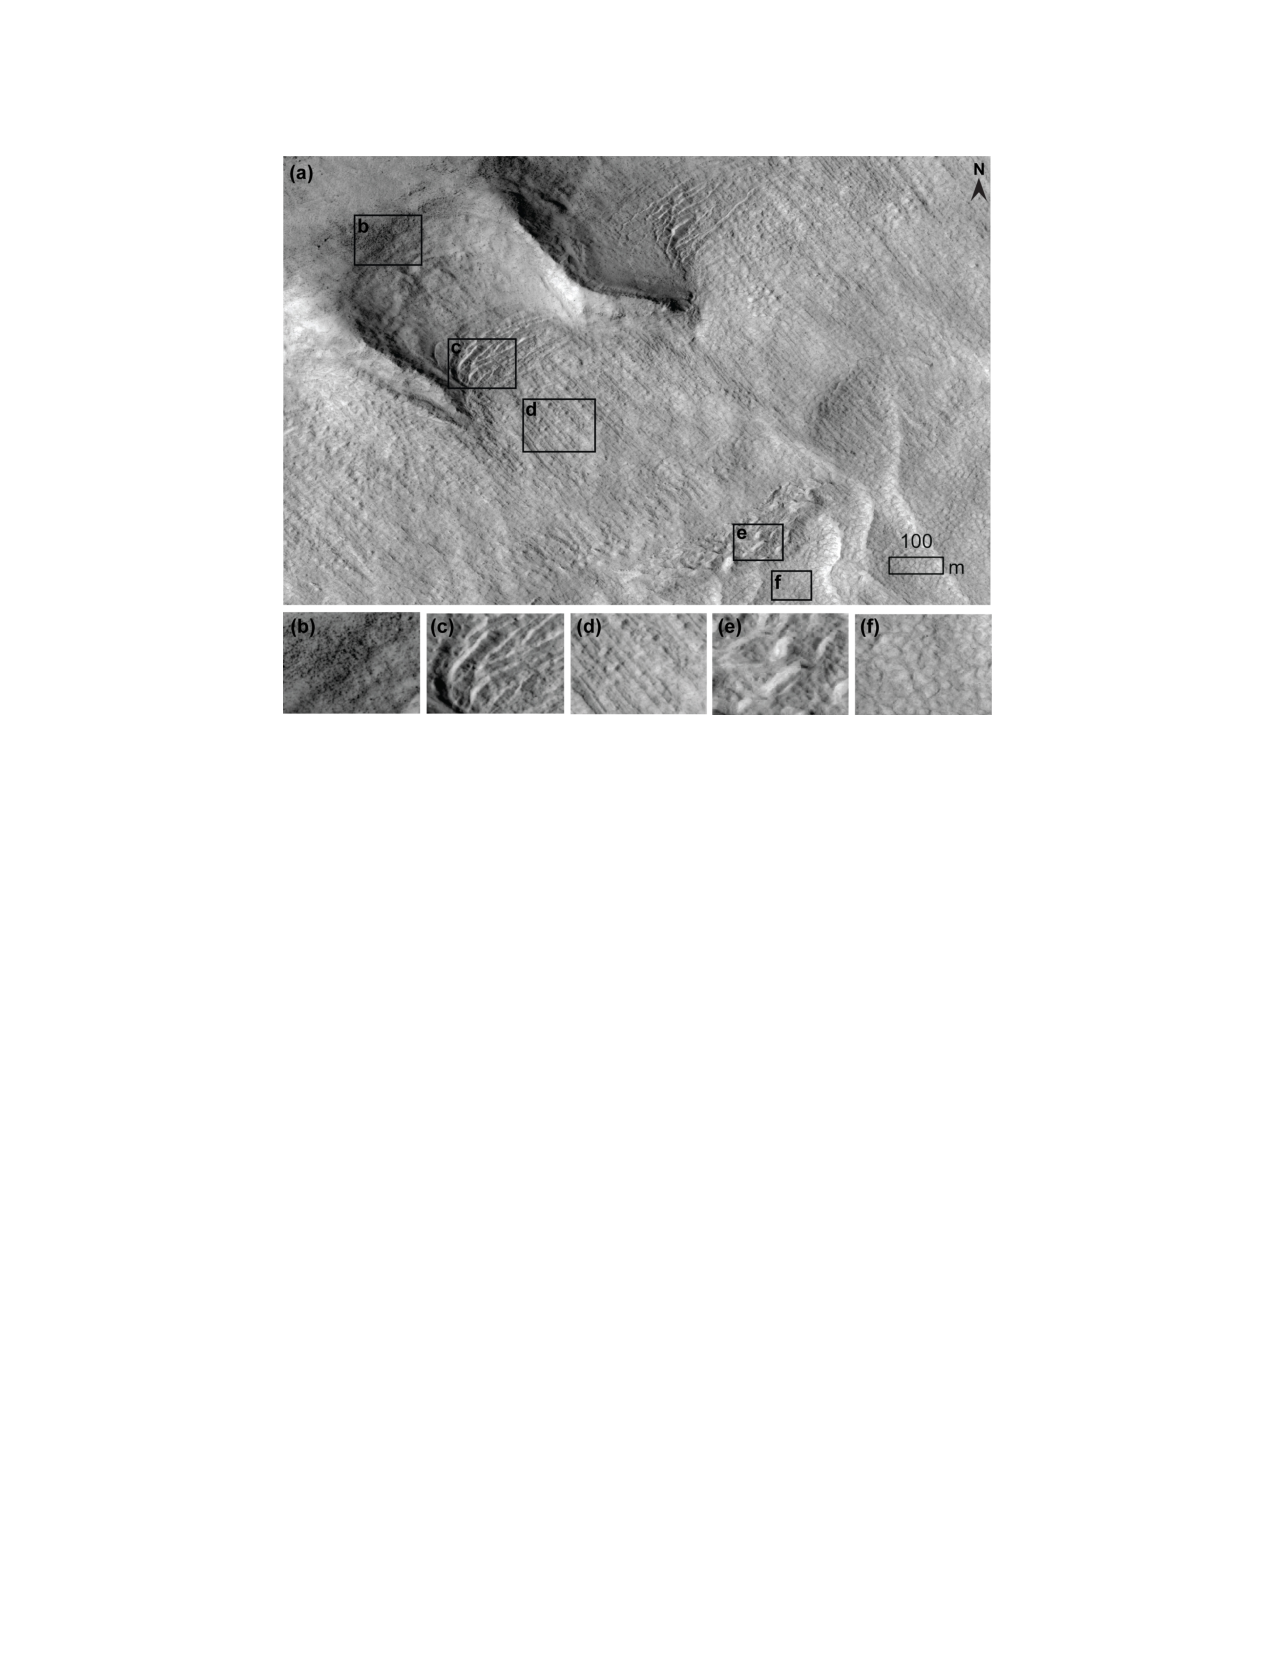
\includegraphics[
    height=0.6\textheight,
    keepaspectratio
]{Figures/Diagrams/Li26_Fig10.pdf}
\caption{HiRISE image data of a cirque-like alcove at Deuteronlius Mensae ($46.57^{\circ}$N, $22.12^{\circ}$E); (b) boulders at top of headwall; (c) washboard terrain; (d) linear terrain; (e) rectilinear ridges; (f) polygonal terrain (Figure from \cite{Li26}).}
\label{fig:Li26}
\end{figure}
\end{frame}

\begin{frame}{GLF Example: Cirque (Corrie)}
    \begin{figure}
    \centering
        \begin{subfigure}{0.48\linewidth}
            \centering
            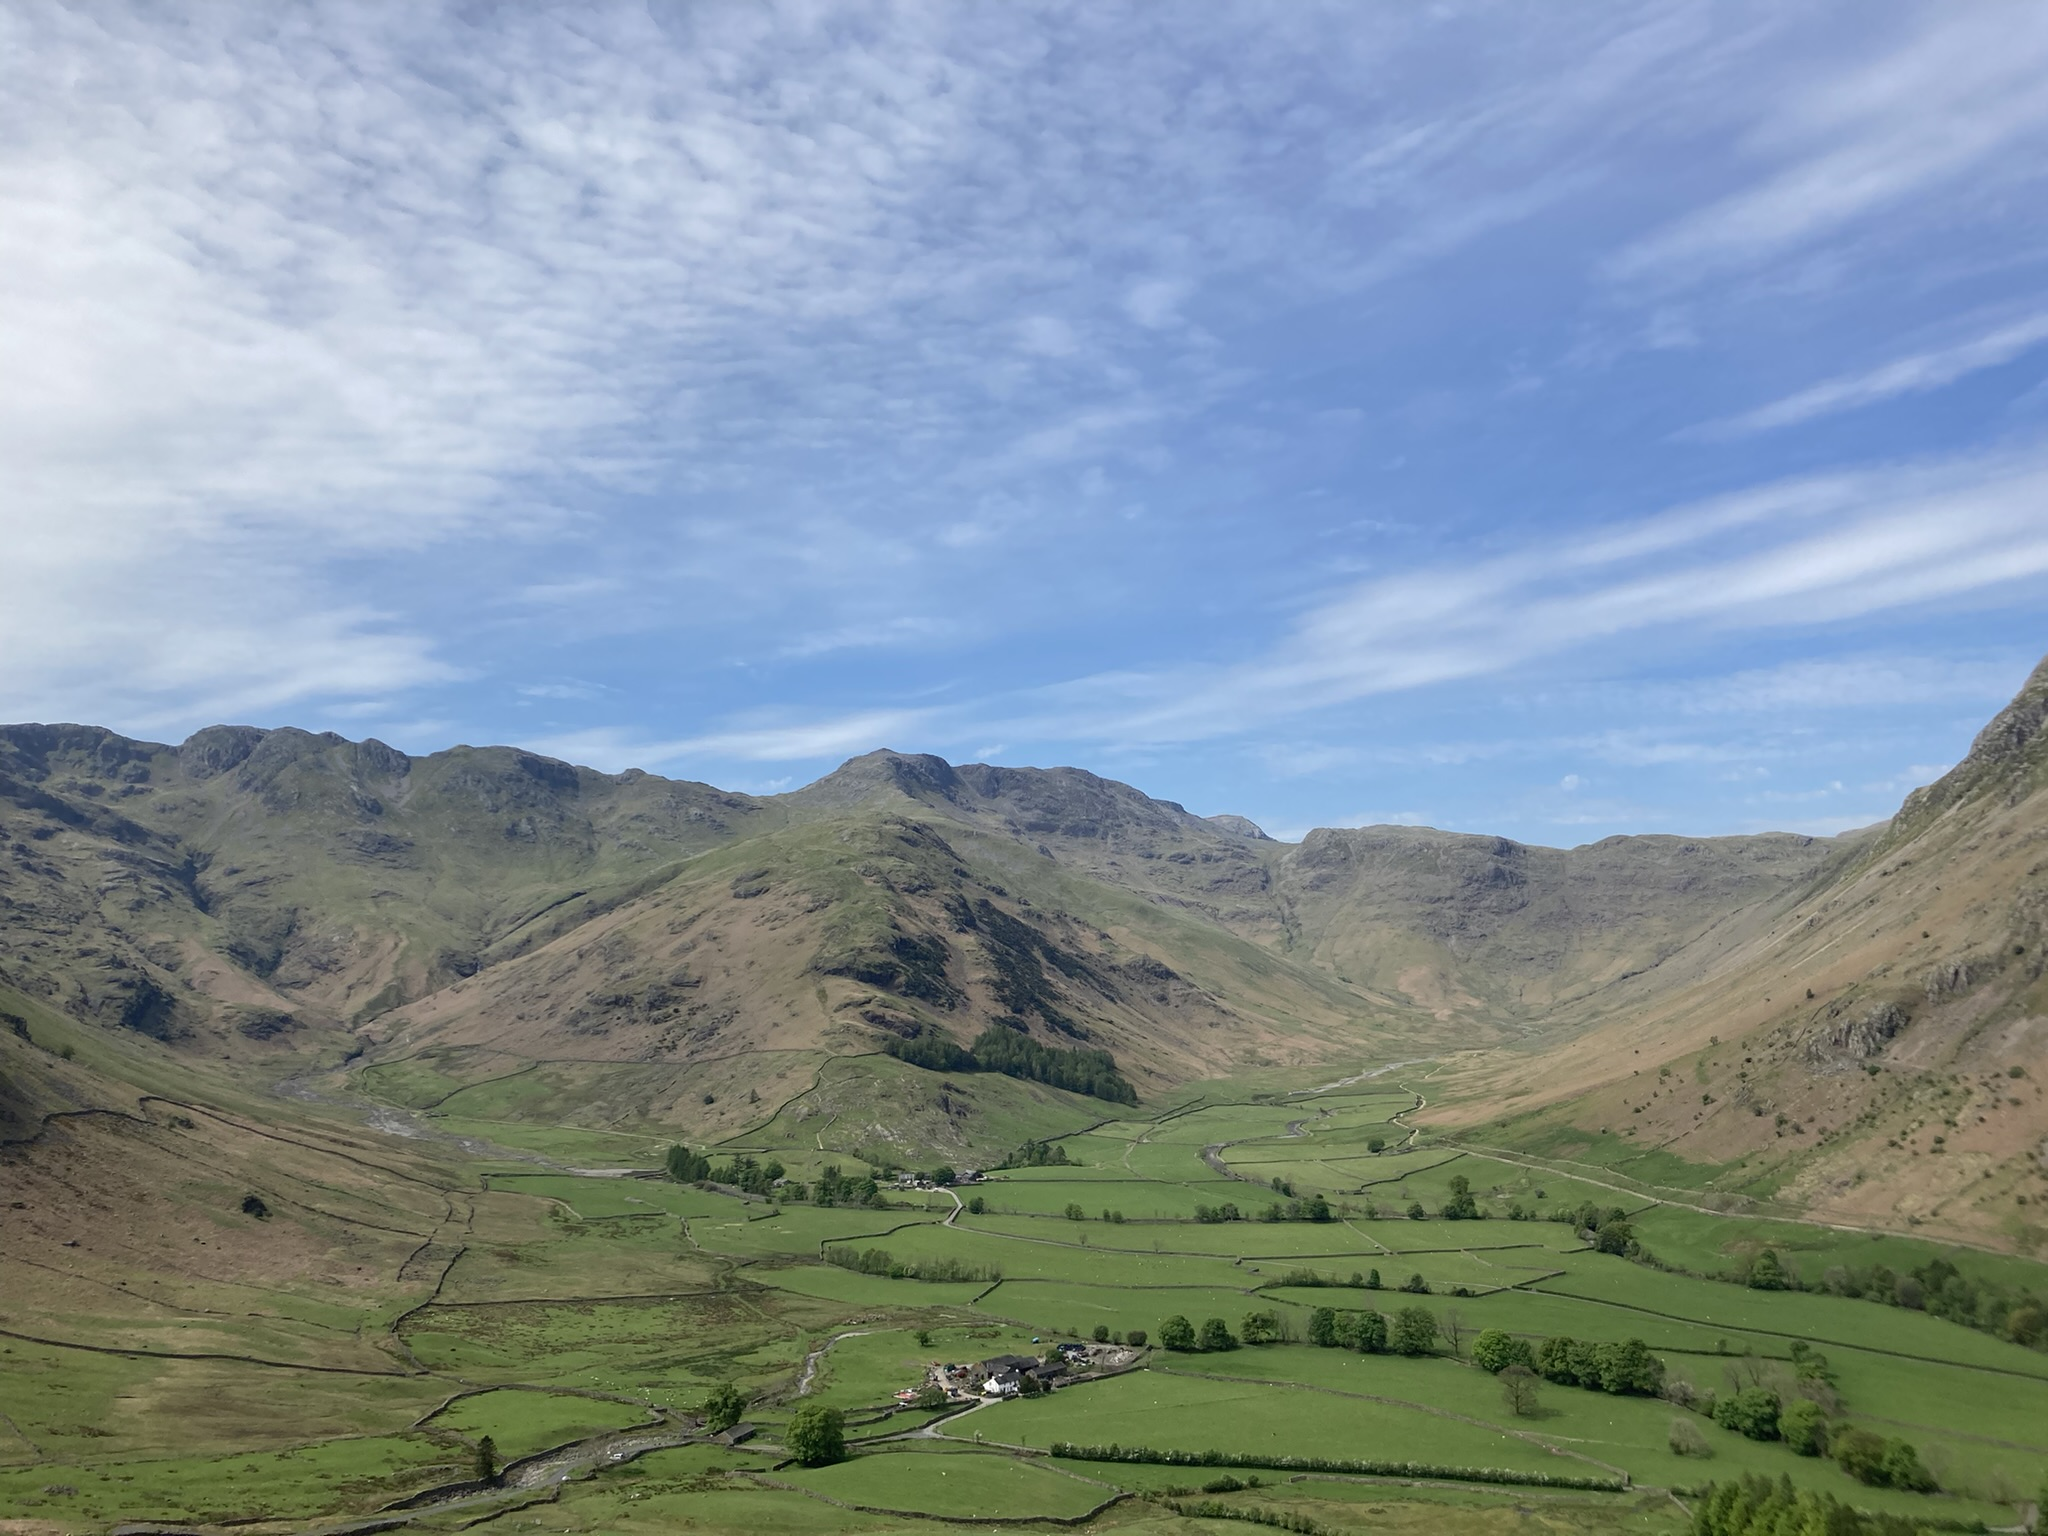
\includegraphics[width=\linewidth]{Figures/Corrie/Langdale_2.jpeg}
            \caption{View looking west from Great Langdale, toward Scafell Pike \(54.50^\circ\ \text{N}\) and \(-2.99^\circ\ \text{E}\).}
            \label{fig:Langdale_2}
        \end{subfigure}
        \hfill
        \begin{subfigure}{0.48\linewidth}
            \centering
            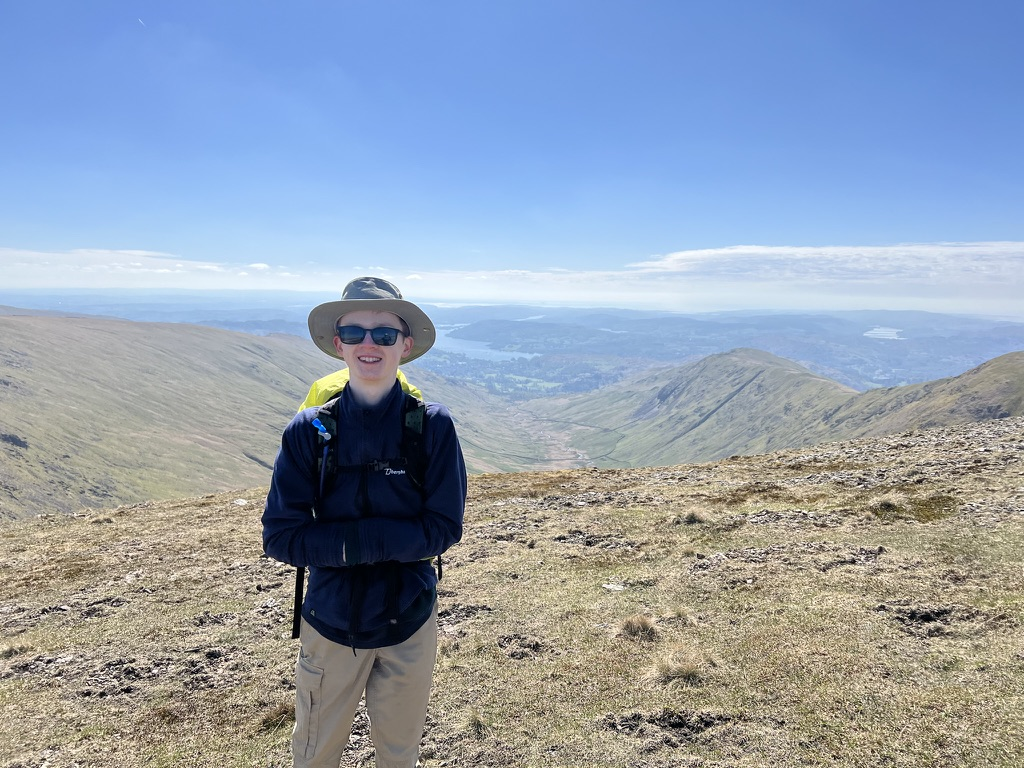
\includegraphics[width=\linewidth]{Figures/Corrie/Langdale_1.jpeg}
            \caption{View looking south from Fairfield over Deepdale.}
            \label{fig:Langdale_1}
        \end{subfigure}
        \caption{Views of corries at in the Lake District.}
        \label{fig:Langdale}
    \end{figure}
\end{frame}